\documentclass{beamer}

\usetheme{UiO}

\usepackage{tikz}

\usetikzlibrary{arrows.meta}

\title{Investigating human cognition with explainable artificial intelligence}
\author{Esten H. Leonardsen}
\date{\today}

\newcommand{\neuron}[3]{
    \node[circle, minimum size=0.3cm, inner sep=0pt, outer sep=0pt, draw=black, fill=#2, anchor=center] (#1) at #3 {};
}

\newcommand{\ann}{
    \def\hsep{0.55}
    \def\vsep{0.45}

    \begin{tikzpicture}
        \neuron{n00}{blue!70}{(-2*\hsep, \vsep)}
        \neuron{n01}{blue!90}{(-2*\hsep, 0)}
        \neuron{n02}{blue!45}{(-2*\hsep, -\vsep)}

        \neuron{n10}{blue!25}{(-\hsep, 2*\vsep)}
        \neuron{n11}{blue!95}{(-\hsep, \vsep)}
        \neuron{n12}{blue!80}{(-\hsep, 0)}
        \neuron{n13}{blue!40}{(-\hsep, -\vsep)}
        \neuron{n14}{blue!75}{(-\hsep, -2*\vsep)}

        \neuron{n20}{blue}{(0, 2*\vsep)}
        \neuron{n21}{blue!15}{(0, \vsep)}
        \neuron{n22}{blue!75}{(0, 0)}
        \neuron{n23}{blue!25}{(0, -\vsep)}
        \neuron{n24}{blue!45}{(0, -2*\vsep)}

        \neuron{n30}{blue!95}{(\hsep, \vsep)}
        \neuron{n31}{blue!40}{(\hsep, 0)}
        \neuron{n32}{blue!60}{(\hsep, -\vsep)}

        \neuron{n40}{blue!75}{(2*\hsep, 0)}

        \def\edgecolour{gray}
        \def\edgeopacity{0.5}

        \draw[\edgecolour, opacity=\edgeopacity] (n00) -- (n10);
        \draw[\edgecolour, opacity=\edgeopacity] (n00) -- (n11);
        \draw[\edgecolour, opacity=\edgeopacity] (n00) -- (n12);
        \draw[\edgecolour, opacity=\edgeopacity] (n00) -- (n13);
        \draw[\edgecolour, opacity=\edgeopacity] (n00) -- (n14);
        \draw[\edgecolour, opacity=\edgeopacity] (n01) -- (n10);
        \draw[\edgecolour, opacity=\edgeopacity] (n01) -- (n11);
        \draw[\edgecolour, opacity=\edgeopacity] (n01) -- (n12);
        \draw[\edgecolour, opacity=\edgeopacity] (n01) -- (n13);
        \draw[\edgecolour, opacity=\edgeopacity] (n01) -- (n14);
        \draw[\edgecolour, opacity=\edgeopacity] (n02) -- (n10);
        \draw[\edgecolour, opacity=\edgeopacity] (n02) -- (n11);
        \draw[\edgecolour, opacity=\edgeopacity] (n02) -- (n12);
        \draw[\edgecolour, opacity=\edgeopacity] (n02) -- (n13);
        \draw[\edgecolour, opacity=\edgeopacity] (n02) -- (n14);

        \draw[\edgecolour, opacity=\edgeopacity] (n10) -- (n20);
        \draw[\edgecolour, opacity=\edgeopacity] (n10) -- (n21);
        \draw[\edgecolour, opacity=\edgeopacity] (n10) -- (n22);
        \draw[\edgecolour, opacity=\edgeopacity] (n10) -- (n23);
        \draw[\edgecolour, opacity=\edgeopacity] (n10) -- (n24);
        \draw[\edgecolour, opacity=\edgeopacity] (n11) -- (n20);
        \draw[\edgecolour, opacity=\edgeopacity] (n11) -- (n21);
        \draw[\edgecolour, opacity=\edgeopacity] (n11) -- (n22);
        \draw[\edgecolour, opacity=\edgeopacity] (n11) -- (n23);
        \draw[\edgecolour, opacity=\edgeopacity] (n11) -- (n24);
        \draw[\edgecolour, opacity=\edgeopacity] (n12) -- (n20);
        \draw[\edgecolour, opacity=\edgeopacity] (n12) -- (n21);
        \draw[\edgecolour, opacity=\edgeopacity] (n12) -- (n22);
        \draw[\edgecolour, opacity=\edgeopacity] (n12) -- (n23);
        \draw[\edgecolour, opacity=\edgeopacity] (n12) -- (n24);
        \draw[\edgecolour, opacity=\edgeopacity] (n13) -- (n20);
        \draw[\edgecolour, opacity=\edgeopacity] (n13) -- (n21);
        \draw[\edgecolour, opacity=\edgeopacity] (n13) -- (n22);
        \draw[\edgecolour, opacity=\edgeopacity] (n13) -- (n23);
        \draw[\edgecolour, opacity=\edgeopacity] (n13) -- (n24);
        \draw[\edgecolour, opacity=\edgeopacity] (n14) -- (n20);
        \draw[\edgecolour, opacity=\edgeopacity] (n14) -- (n21);
        \draw[\edgecolour, opacity=\edgeopacity] (n14) -- (n22);
        \draw[\edgecolour, opacity=\edgeopacity] (n14) -- (n23);
        \draw[\edgecolour, opacity=\edgeopacity] (n14) -- (n24);

        \draw[\edgecolour, opacity=\edgeopacity] (n20) -- (n30);
        \draw[\edgecolour, opacity=\edgeopacity] (n20) -- (n31);
        \draw[\edgecolour, opacity=\edgeopacity] (n20) -- (n32);
        \draw[\edgecolour, opacity=\edgeopacity] (n21) -- (n30);
        \draw[\edgecolour, opacity=\edgeopacity] (n21) -- (n31);
        \draw[\edgecolour, opacity=\edgeopacity] (n21) -- (n32);
        \draw[\edgecolour, opacity=\edgeopacity] (n22) -- (n30);
        \draw[\edgecolour, opacity=\edgeopacity] (n22) -- (n31);
        \draw[\edgecolour, opacity=\edgeopacity] (n22) -- (n32);
        \draw[\edgecolour, opacity=\edgeopacity] (n23) -- (n30);
        \draw[\edgecolour, opacity=\edgeopacity] (n23) -- (n31);
        \draw[\edgecolour, opacity=\edgeopacity] (n23) -- (n32);
        \draw[\edgecolour, opacity=\edgeopacity] (n24) -- (n30);
        \draw[\edgecolour, opacity=\edgeopacity] (n24) -- (n31);
        \draw[\edgecolour, opacity=\edgeopacity] (n24) -- (n32);

        \draw[\edgecolour, opacity=\edgeopacity] (n30) -- (n40);
        \draw[\edgecolour, opacity=\edgeopacity] (n31) -- (n40);
        \draw[\edgecolour, opacity=\edgeopacity] (n32) -- (n40);

    \end{tikzpicture}
}
\newcommand{\behaviournode}[3]{
	\node[draw=black, minimum height=0.2cm, minimum width=0.5cm, inner sep=0pt, outer sep=0pt, #2] (#1) at #3 {};
}

\begin{document}
	\begin{frame}
	 	\titlepage
	\end{frame}

	\begin{frame}{}
		\def\xmin{-6.45}
		\def\xmax{6.45}
		\def\ymin{-3.15}
		\def\ymax{3.15}

		\begin{tikzpicture}
			\node[draw=black, anchor=north west, outer sep=0pt] at (\xmin, \ymax) {};
			\node[draw=black, anchor=south east, outer sep=0pt] at (\xmax, \ymin) {};

			\node[anchor=north west, outer sep=0pt, inner sep=0pt, draw=black, fill=gray] (brain) at (\xmin, \ymax) {
				\scalebox{-1}[1]{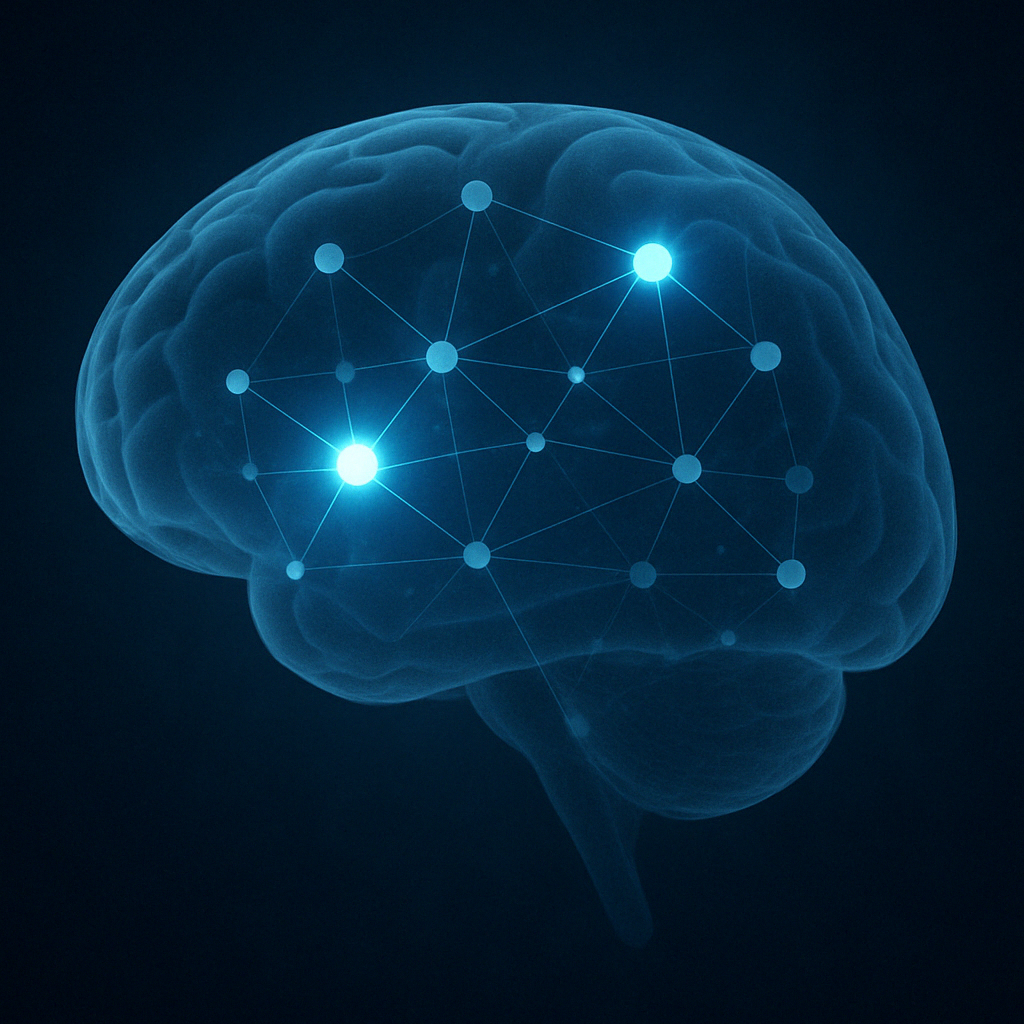
\includegraphics[width=3cm]{data/workingbrain.png}}
			};
			\node[anchor=south east, text=white, font=\Large\bfseries] at (brain.south east) {a};

			\node[anchor=south west, minimum height=2cm, minimum width=3cm, inner sep=0pt, outer sep=0pt] (behaviour) at (\xmin, \ymin) {};
			\behaviournode{b0}{solid}{($ (behaviour.north) - (1.05, 0.4) $)};
			\behaviournode{b1}{solid}{($ (behaviour.north) - (0.3, 0.4) $)};
			\behaviournode{b2}{solid}{($ (behaviour.north) - (-0.9, 0.4) $)};
			\draw[] ($ (behaviour.north west) + (0.1, -0.4) $) -- (b0) -- (b1) -- (b2) -- ($ (behaviour.north east) + (-0.1, -0.4) $);
			\draw[-Latex] ($ (behaviour.north west) + (0.1, -1) $) -- ($ (behaviour.north east) + (-0.1, -1) $);
			\node[] at ($ (behaviour.north) - (0, 1.3) $) {Time};
			\node[anchor=south east, font=\Large\bfseries] at (behaviour.south east) {b};

			\node[anchor=north, draw=black, inner sep=0pt] (eeg) at (0, \ymax) {
				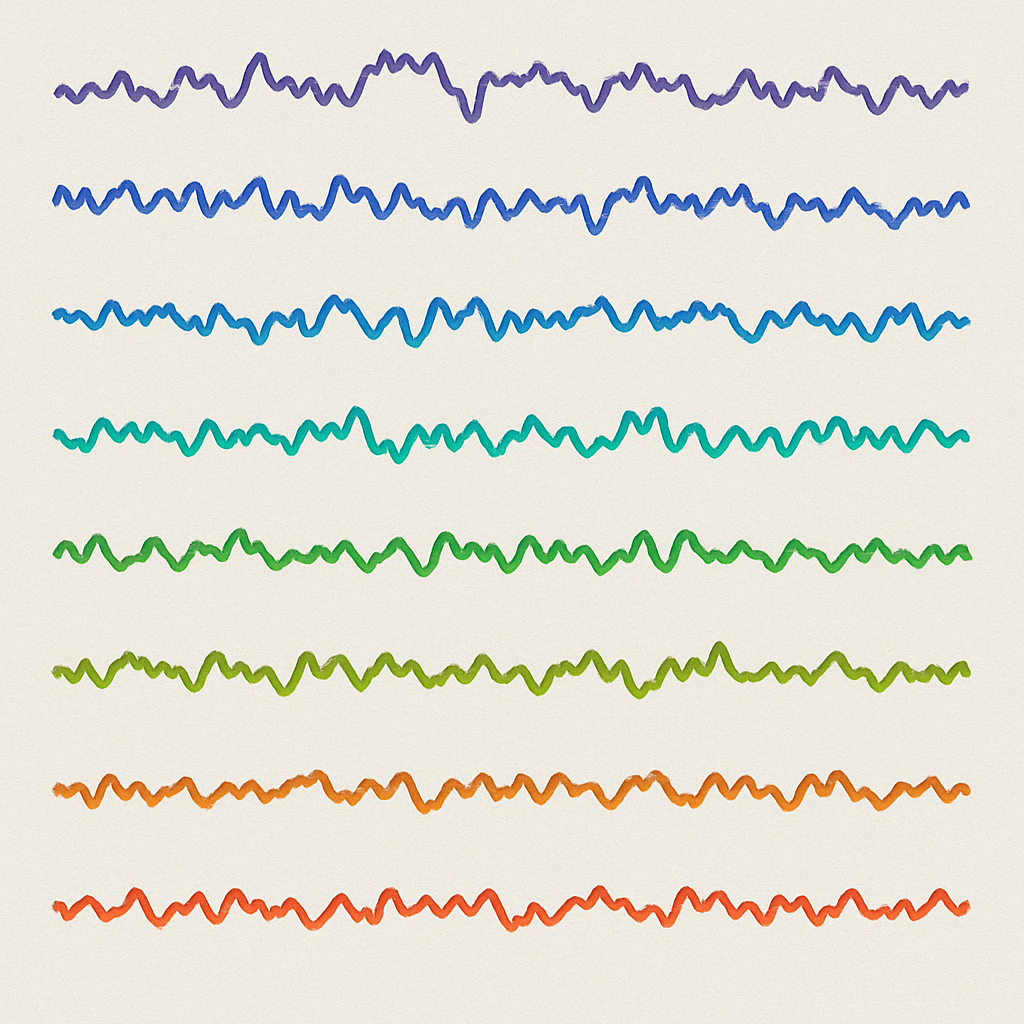
\includegraphics[width=3cm]{data/eeg.png}
			};
			\node[anchor=south east, font=\Large\bfseries] at (eeg.south east) {c};

			\node[anchor=north east, minimum height=3cm, minimum width=3cm, inner sep=0pt, outer sep=0pt] (ann) at (\xmax, \ymax) {
				\ann
			};
			\node[anchor=south east, font=\Large\bfseries] at (ann.south east) {d};

			\node[anchor=south east, minimum height=2cm, minimum width=3cm, inner sep=0pt, outer sep=0pt] (prediction) at (\xmax, \ymin) {};
			\behaviournode{p0}{densely dotted}{($ (prediction.north) - (1, 0.4) $)};
			\behaviournode{p1}{densely dotted}{($ (prediction.north) - (0.4, 0.4) $)};
			\behaviournode{p2}{densely dotted}{($ (prediction.north) - (-0.7, 0.4) $)};

			\draw[densely dotted] ($ (prediction.north west) + (0.1, -0.4) $) -- (p0) -- (p1) -- (p2) -- ($ (prediction.north east) + (-0.1, -0.4) $);
			\draw[-Latex] ($ (prediction.north west) + (0.1, -1) $) -- ($ (prediction.north east) + (-0.1, -1) $);
			\node[] at ($ (prediction.north) + (0, -1.3) $) {Time};
			\node[anchor=south east, font=\Large\bfseries] at (prediction.south east) {e};

			\draw[-{Stealth[length=10pt, width=16pt]}, line width=10pt, gray] (brain) -- (eeg) node[midway, text=black, text=white, font=\fontsize{6}{4}\selectfont, text depth=0] {Record};
			\draw[-{Stealth[length=10pt, width=16pt]}, line width=10pt, gray] (brain) -- (behaviour) node[midway, text=black, text=white, font=\fontsize{6}{4}\selectfont, rotate=270, text depth=0] {Solve};
			\draw[-{Stealth[length=10pt, width=16pt]}, line width=10pt, gray] (eeg) -- (ann) node[midway, text=black, text=white, font=\fontsize{6}{4}\selectfont, text depth=0] {Analyze};
			\draw[-{Stealth[length=10pt, width=16pt]}, line width=10pt, gray] ($ (ann.south) - (0.3, 0) $) -- ($ (prediction.north) - (0.3, 0) $) node[midway, text=black, rotate=270, text=white, font=\fontsize{6}{4}\selectfont, text depth=0] {Predict};
			\draw[-{Stealth[length=10pt, width=16pt]}, line width=10pt, gray] ($ (prediction.north) + (0.3, 0) $) -- ($ (ann.south) + (0.3, 0) $) node[midway, text=black, rotate=90, text=white, font=\fontsize{6}{4}\selectfont, text depth=0] {Explain};
			\draw[{Stealth[length=10pt, width=16pt]}-{Stealth[length=10pt, width=16pt]}, line width=10pt, gray] ($ (behaviour.east) + (0, 0.6) $) -- ($ (prediction.west) + (0, 0.6) $) node[midway, text=black, text=white, font=\fontsize{6}{4}\selectfont, text depth=0] {Compare};
			\draw[{Stealth[length=10pt, width=16pt]}-{Stealth[length=10pt, width=16pt]}, line width=10pt, gray] (brain.north) |- ($ (eeg.north) + (0, 0.75) $) -| (ann.north);
			\node [text=white, font=\fontsize{6}{4}\selectfont, text depth=0] at ($ (eeg.north) + (0, 0.75) $) {Align};

		\end{tikzpicture}
	\end{frame}

\end{document}
